\documentclass[onecolumn, draftclsnofoot,10pt, compsoc]{IEEEtran}
\usepackage{graphicx}
\usepackage{url}
\usepackage{setspace}
\usepackage{times}
\usepackage{enumitem}
\usepackage{titletoc}
\usepackage{float}
\usepackage{listings}
\usepackage{caption}
%\usepackage[export]{adjustbox}
%\usepackage[notocbib]{apacite}
\usepackage{geometry}
\geometry{textheight=9.5in, textwidth=7in}

% 1. Fill in these details
\def \CapstoneTeamName{		Beached Marine Critters Project Team}
\def \CapstoneTeamNumber{		64}
\def \GroupMemberOne{			Alea Weeks}
\def \GroupMemberTwo{			Amar Raad}
\def \GroupMemberThree{			Daniel Domme}
\def \GroupMemberFour{			Justin Disalvo}
\def \GroupMemberFive{			Zachary Tusing}
\def \CapstoneProjectName{		Develop a visual model for sea turtle beach stranding Events}
\def \CapstoneSponsorCompany{	Oregon State University Hatfield Marine Science Center; Oregon Sea Grant}
\def \CapstoneSponsorPerson{		Dr. William Hanshumaker}

% 2. Uncomment the appropriate line below so that the document type works
\def \DocType{		%Problem Statement
				%Requirements Document
				%Technology Review
				%Design Document
				Progress Report
				}
			
\newcommand{\NameSigPair}[1]{\par
\makebox[2.75in][r]{#1} \hfil 	\makebox[3.25in]{\makebox[2.25in]{\hrulefill} \hfill		\makebox[.75in]{\hrulefill}}
\par\vspace{-12pt} \textit{\tiny\noindent
\makebox[2.75in]{} \hfil		\makebox[3.25in]{\makebox[2.25in][r]{Signature} \hfill	\makebox[.75in][r]{Date}}}}
% 3. If the document is not to be signed, uncomment the RENEWcommand below
\renewcommand{\NameSigPair}[1]{#1}
\doublespacing
%%%%%%%%%%%%%%%%%%%%%%%%%%%%%%%%%%%%%%%
\begin{document}
\begin{titlepage}
    \pagenumbering{gobble}
    \begin{singlespace}
     \includegraphics[height=3cm]{coe_v_spot1}
        \hfill 
        % 4. If you have a logo, use this includegraphics command to put it on the coversheet.
        %\includegraphics[height=4cm]{CompanyLogo}   
        \par\vspace{.2in}
        \centering
        \scshape{
            \huge CS Capstone \DocType \par
            {\normalsize\today}\par
            \vspace{.5in}
            \textbf{\Huge\CapstoneProjectName}\par
            %\vfill
            \vspace{1in}
            {\Large Prepared for}\par
            \huge \CapstoneSponsorCompany\par
            \vspace{5pt}
            {\Large\NameSigPair{\CapstoneSponsorPerson}\par}
            \vspace{.5in}
            {\large Prepared by }\par
            Group\CapstoneTeamNumber\par
            % 5. comment out the line below this one if you do not wish to name your team
            %\CapstoneTeamName\par 
            \vspace{5pt}
            {\Large
                \NameSigPair{\GroupMemberOne}\par
                \NameSigPair{\GroupMemberTwo}\par
                \NameSigPair{\GroupMemberThree}\par
				\NameSigPair{\GroupMemberFour}\par
			\NameSigPair{\GroupMemberFive}\par
            }
            \vspace{20pt}
        }
        \vfill
        \begin{abstract}
        % 6. Fill in your abstract    
        	%This document is written using one sentence per line.
        	%This allows you to have sensible diffs when you use \LaTeX with version control, as well as giving a quick visual test to see if sentences are too short/long.
        	%If you have questions, ``The Not So Short Guide to LaTeX'' is a great resource (\url{https://tobi.oetiker.ch/lshort/lshort.pdf})
		    \noindent This document is a summary of all activities that took place during this term and the current state of the project. The outline of problems, possible solutions, and learned is also discussed.
		    
        \end{abstract}     
    \end{singlespace}
\end{titlepage}
\newpage
\pagenumbering{arabic}
\tableofcontents
% 7. uncomment this (if applicable). Consider adding a page break.
%\listoffigures
%\listoftables
\clearpage
%\begin{singlespace}

\section{Project Purpose and Goals}
The purpose of the beached marine critters project is to use archival data to create a visual model of sea turtle beach stranding events. The archival data will include information about the beached animal as well as sea conditions such as sea surface temperature, currents and wind direction. The ultimate purpose is to use the visual model to draw correlations between preexisting ocean conditions and the dates of sea turtle stranding events. The goal is to gain understanding of how oceanographic conditions lead to stranded animals aid in the timely rescue of sea turtles.

\section{Current State of Project}
\subsection{ArcGIS and Data Collection - Alea and Daniel}
We have made good progress on creating a visual representation of stranded sea turtle and sea condition data.
We have gathered historical data from the years 1957 - 2018 on sea conditions for the Pacific Northwest Coast. We have a database with over 54 million unique rows representing historical weather data for each day from the year 1957 until 2018. We will use this data to calculate daily averages and create map layers from this. The data are standardized to match the format of the beached sea turtle data. We have imported the sea turtle data into ArcGIS (mapping and data analysis software) and have visually represented this data on the map. This is shown in Figure 1. \newline \newline

\begin{figure}[H]
  \includegraphics[scale=0.55]{turtle_data.JPG}
  \caption{Sea turtle data plotted on a map}
\end{figure}

The next couple of screenshots give examples of how our data looks when overlapped.  \newline

\begin{figure}[H]
  \includegraphics[scale=0.55]{sea_surface_idw_and_wind_map.JPG}
  \caption{Wind velocity and sea surface temperature map layers}
\end{figure}

\begin{figure}[H]
  \includegraphics[scale=0.55]{air_temp_and_wind_current.JPG}
  \caption{Wind velocity and air temperature map layers}
\end{figure}

\subsection{GUI - Justin and Zach}
This project's UI needed to provide simple functionalities and be easily manipulable for the rest of our team. The UI was designed with simplicity in mind so that researchers and inexperienced users would easily be able to understand what is going on. The UI has simple button outline for easy access to our different functions. We've been working to provide a larger base of functionality most of the term so that the rest of the team can start working on the background functions and implementing them for the GUI. We are not satisfied with the look of the GUI and are intending to provide a better look and feel to everything about our UI. This means that we will provide a simple yet beautiful GUI.

\subsection{Integration - Amar}

Upon complete integration, the recorded locations of sea turtle strandings should be able to display on the map implemented into the GUI. Selecting "From" and "To" timestamps should then call for the time period of all recordings found in-between the two. When calling for this function, the GUI should access and retrieve data from the ArcGIS map, selecting the appropriate data to be displayed for the user. Although the integration between the ArcGIS map and GUI is still in process, once the GUI can successfully pull and display data from a static timestamp of data, then toggling along different timestamps with the live data should be next to implement.

\section{What Needs to Be Done}

\subsection{ArcGIS and Data Collection - Alea and Daniel} 
\par We need to condense our data set to only include data that will be meaningful to the project. For example, currently we have daily sea condition data for years when there was not a single sea turtle stranding. The sea condition data that we currently have includes recordings every few hours of every day between 1957 and 2018. This is too much data. One way of slimming the data down would be to just have daily averages.  We also need to adjust the data map layers to be easily viewed at the same time.
\par The ocean current data needs to be standardized to make vectors on the map.  The format that it is currently in will not work effectively.

\par Visually there is a lot of little improvements we still need to make to the map. For example, in Figures 2 and 3 a lot of sea condition data has been interpolated and includes average sea data on land. To fix this we need to limit the sea condition data to only be plotted on sea and not on land. Other visual improvements will be made after our client reviews our work and provides feedback. 

\subsection{GUI - Justin and Zach}
\par The GUI is very basic, so far. All the buttons are present and the structure of the GUI is complete. All that is left is making it look nicer and making any changes that may need to be made based on the integration of ArcGIS. One of these changes will be the Data section to the right of the map. This will be created based on the number of sea turtles that are in the imported file.
\newline \newline
\includegraphics[scale=0.6]{current-ui.PNG}
\subsection{Integration - Amar}
The GUI still needs to be able to successfully access our sets of data. In a test process the GUI could access a public example ArcGIS map and display the corresponding location points of it. Some variables will need to be changed along with implementing readability access to our database and ArcGIS map so that the GUI may have the desired and working functionality.

\section{Problems and Solutions}
\subsection{ArcGIS and Data}
During the initial weeks of this term, multiple members of the team had problems getting access to ArcGIS software license. 

\par A roadblock that was faced by the team in gathering data from government sources early in the term was the government shutdown.  Many agencies that collected and published data sets for weather and sea conditions were not operating. The websites were not accessible for a few weeks.  This caused a disruption in the amount of work that could be done with processing and mapping data.  Fortunately, after the shutdown ended, the websites were operational in shortly after, and the necessary data could be gathered.\newline

A problem with the data for our project is that the amount of weather data that was collected is immense in volume.  There are over 54 million unique lines of weather entries.  This poses a problem with the stability of the ArcGIS software, which, when overloaded with computations, crashes or slows down to unusable speeds.  There are possible solutions that we have to solve this. One solution is to gather a different set of data that only includes daily averages instead of weather conditions throughout the day.  Another solution might be to restrict weather data to days or months surrounding a stranding event.  A final solution might be to go through the data that has been collected and process it to reduce redundant entries and form averages between entries.

\subsection{GUI}
The code to make the GUI is very confusing. We used QtDesigner to create it, and it automatically converts it to a python file. Going through the code and properly commenting and spacing it out will help everyone understand it better. Next, is addressing the Data portion to the right of the map. This will be created when the file is imported. A button will be created for each point on the map, and will be linked to highlight the point on the map when clicked.
\subsection{Integration}
There still is a roadblock in accessing our ArcGIS database. Initially, I also had difficulties acquiring a full licence to the ArcGIS software, so any testing was done with public example maps and locations. However, I was recently able to obtain assistance in acquiring the needed access so I will be able to view and test the integration with a static set of data.

\section{Interesting Code (Zach and Justin)}
Using QtDesigner showed us an interesting way to create a UI. QtDesigner, when converted to a python file, will create everything in an init class then change the value later using a translate function. The first image is what the code looks like in the init function. This is only for the menu bar buttons and drop downs.
\newline \newline

\includegraphics[scale= 1]{intersting-code-1.PNG}
\newline
The next picture is the code that will change the name of the initialized values to what they should be. This is done in a separate function from the init function.
\newline \newline
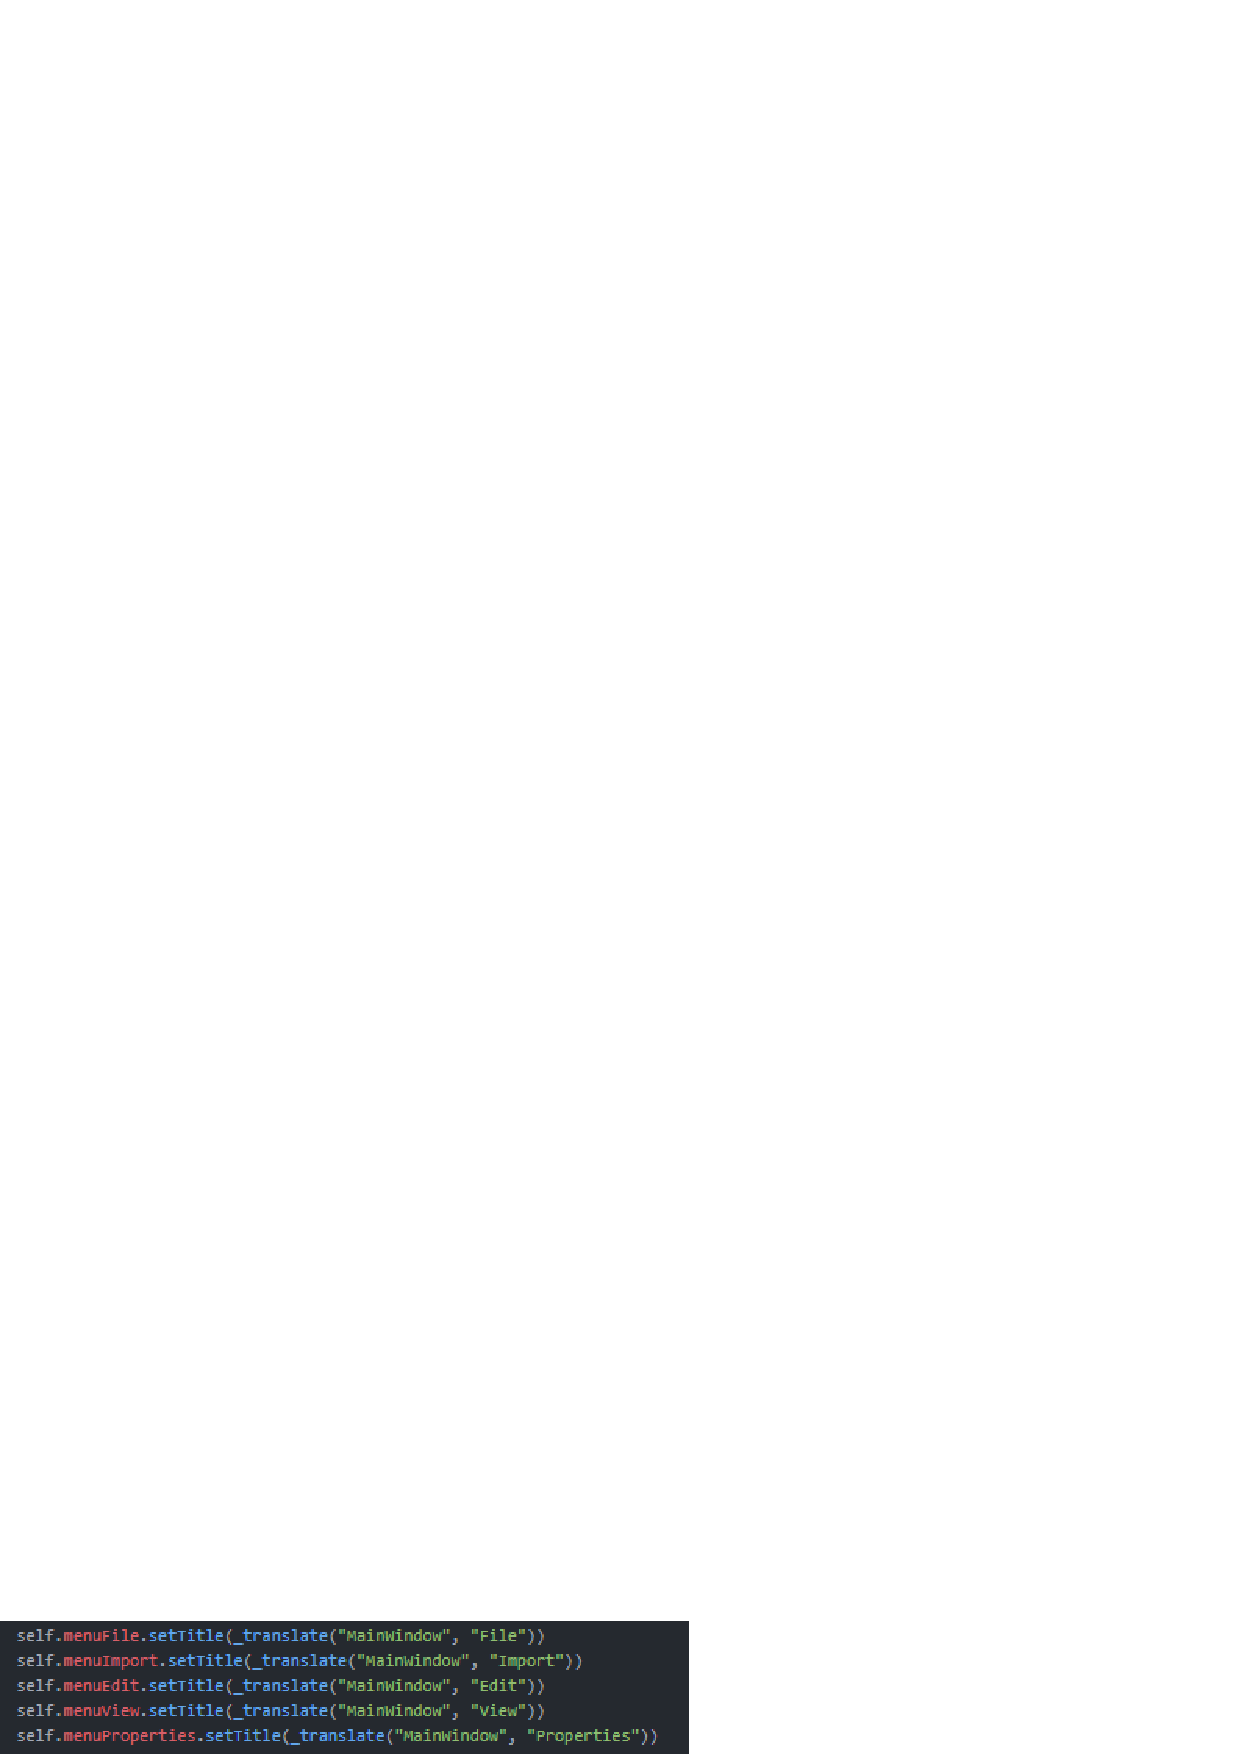
\includegraphics[scale= 1]{intersting-code-2.PNG}
\newline
Before using QtDesigner, we initialized and named everything in the same function.
Our code has generally has some cool implmentation parts. There are lots of neat little small tricks in python to be able to design the UI in the way that one wants. \code{w.setWindowFlags(QtCore.Qt.FramelessWindowHint)} is a good example of how neat the python UI code can be. This snippet of code allows our program to remove the default boarder around the program and implement our own boarder.


\section{Description of First User Study}
We are waiting on Amar to integrate the GUI and our ArcGIS project. No user study has been conducted yet.
When our project is integrated, we will conduct a user study. In this study we will have user's evaluate our GUI and see if there are any clarity improvements that could be made. 

\renewcommand\refname{Bibliography}

% bibliography
\pagebreak
\nocite{*}%if nothing is referenced it will still show up in refs
\bibliographystyle{IEEEtran}
\bibliography{refs}

%\end{singlespace}
\end{document}